\documentclass{article}
\usepackage{graphicx}
\usepackage{subcaption}
\usepackage{geometry}
\usepackage{hyperref}
\usepackage{grffile} % To handle dots and special characters in filenames

\geometry{
    a4paper,
    margin=0.8in
}

\hypersetup{
    colorlinks=true,
    linkcolor=blue,
    filecolor=magenta,      
    urlcolor=cyan,
}

\title{Byzantine Robustness Comparison:\\CNN vs. SNN Encodings (Complete Sweeps)}
\author{ByzFL SNN Benchmark}
\date{\today}

\begin{document}

\maketitle

\tableofcontents
\newpage

\section{Introduction}
This document presents comparison grids (2x2 layout) of Byzantine robustness results for CNN and SNN architectures under different data encoding schemes. The configurations compared are:
\begin{enumerate}
    \item \textbf{CNN}: Convolutional Neural Network on MNIST (`cnn\_complete\_plots`)
    \item \textbf{SNN Rate}: Spiking Neural Network with Rate encoding on MNIST (`snn\_complete\_plots\_rate`)
    \item \textbf{SNN Direct}: Spiking Neural Network with Direct encoding on MNIST (`snn\_complete\_plots\_direct`)
    \item \textbf{SNN NMNIST}: Spiking Neural Network on neuromorphic NMNIST (`snn\_complete\_plots\_nmnist`)
\end{enumerate}

Each grid illustrates the test accuracy under varying numbers of Byzantine clients ($f \in [0, 2, 4, 6]$) and data heterogeneity levels ($\gamma \in [0.0, 0.33, 0.66, 1.0]$).

\newpage

\section{Best Overall (Worst-Case Across All Attacks)}
\label{sec:best_overall}

Figure~\ref{fig:best_overall} compares the best-performing aggregators under the worst-case attack scenario (minimizing the maximum damage over all attacks).

\begin{figure}[htbp]
    \centering
    \begin{subfigure}[b]{0.49\textwidth}
        \centering
        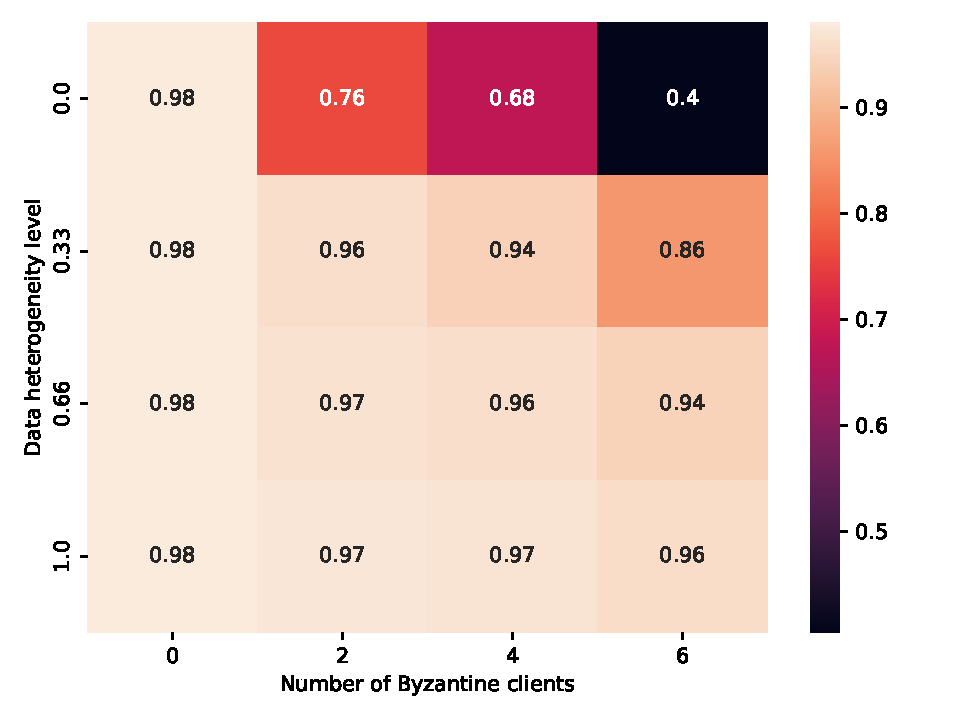
\includegraphics[width=\textwidth]{cnn_complete_plots/best_test_mnist_convnet_cnn_gamma_similarity_niid_NNM_ARC_nb_honest_clients_16_tolerated_f_equal_real.pdf}
        \caption{CNN (Best Overall)}
        \label{fig:overall_cnn}
    \end{subfigure}
    \hfill
    \begin{subfigure}[b]{0.49\textwidth}
        \centering
        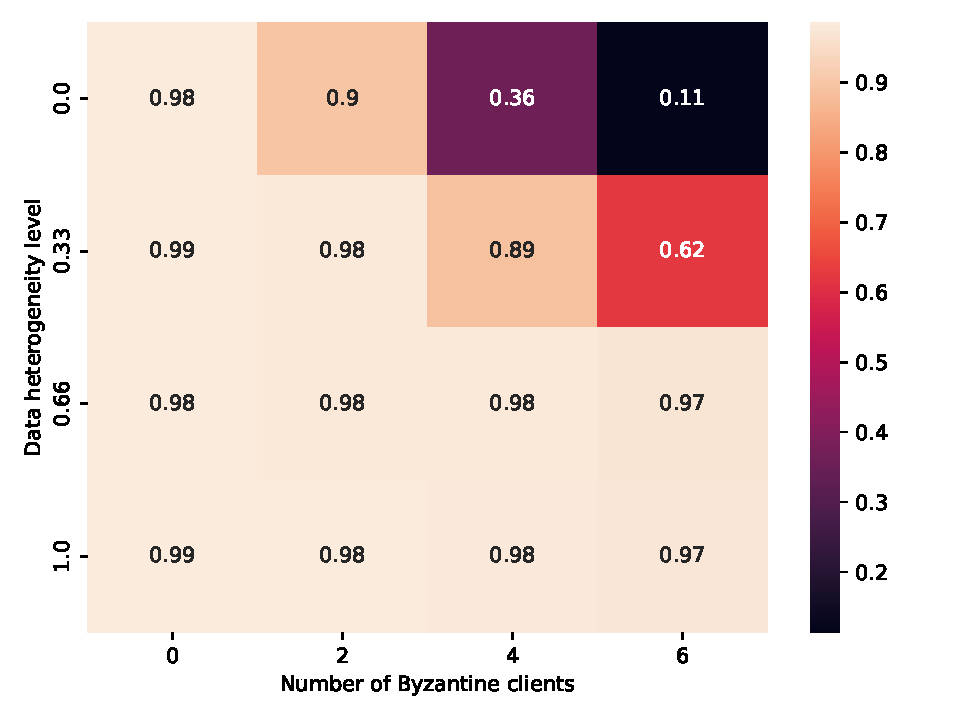
\includegraphics[width=\textwidth]{snn_complete_plots_rate/best_test_mnist_convnet_snn_gamma_similarity_niid_NNM_ARC_nb_honest_clients_16_tolerated_f_equal_real.pdf}
        \caption{SNN Rate (Best Overall)}
        \label{fig:overall_snn_rate}
    \end{subfigure}
    
    \vspace{15pt}
    
    \begin{subfigure}[b]{0.49\textwidth}
        \centering
        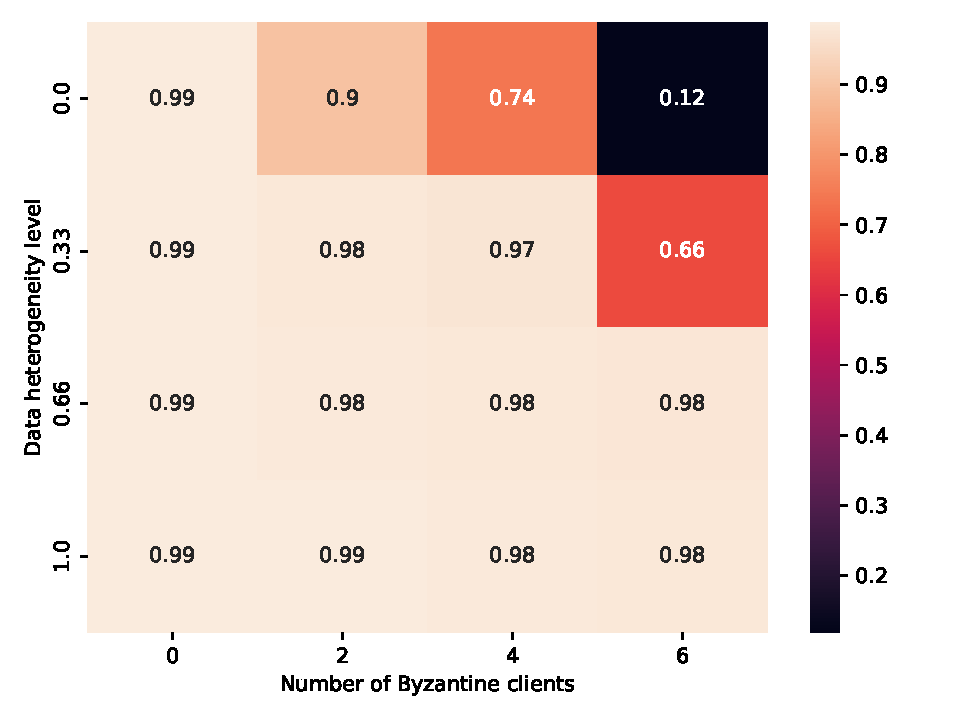
\includegraphics[width=\textwidth]{snn_complete_plots_direct/best_test_mnist_convnet_snn_gamma_similarity_niid_NNM_ARC_nb_honest_clients_16_tolerated_f_equal_real.pdf}
        \caption{SNN Direct (Best Overall)}
        \label{fig:overall_snn_direct}
    \end{subfigure}
    \hfill
    \begin{subfigure}[b]{0.49\textwidth}
        \centering
        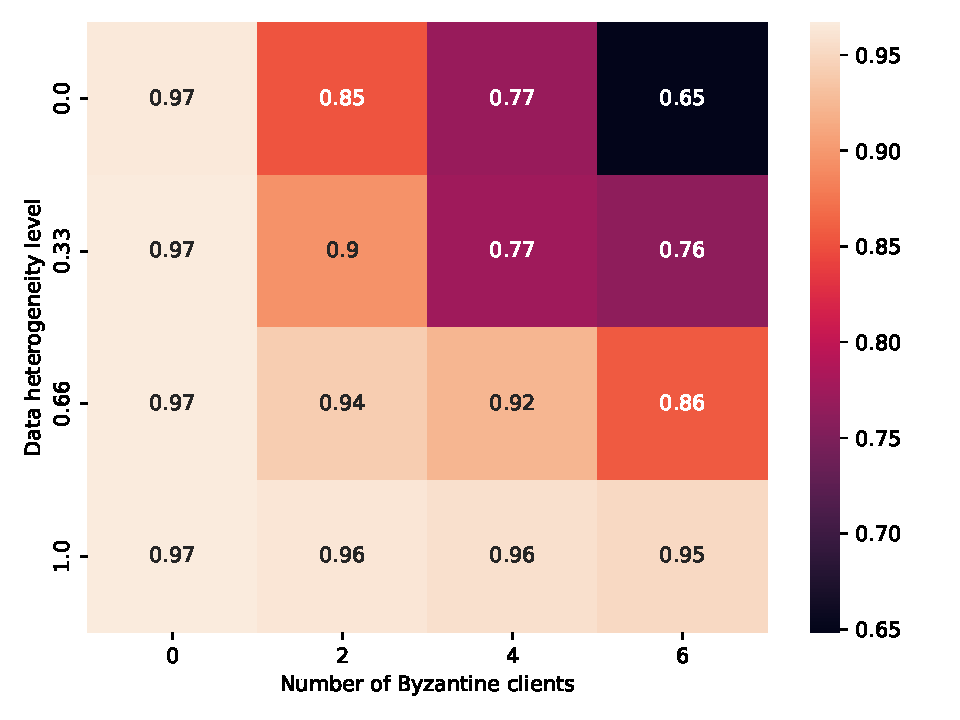
\includegraphics[width=\textwidth]{snn_complete_plots_nmnist/best_test_nmnist_nmnist_snn_gamma_similarity_niid_NNM_ARC_nb_honest_clients_16_tolerated_f_equal_real.pdf}
        \caption{SNN NMNIST (Best Overall)}
        \label{fig:overall_snn_nmnist}
    \end{subfigure}
    \caption{Best overall test accuracy comparison under worst-case attack across different data distribution parameters and number of Byzantine clients.}
    \label{fig:best_overall}
\end{figure}

\newpage

\section{Fixed Attack: Gaussian Noise}
\label{sec:gaussian_attack}

Figure~\ref{fig:gaussian_attack} compares performance when the network is subjected to a Gaussian Byzantine attack.

\begin{figure}[htbp]
    \centering
    \begin{subfigure}[b]{0.49\textwidth}
        \centering
        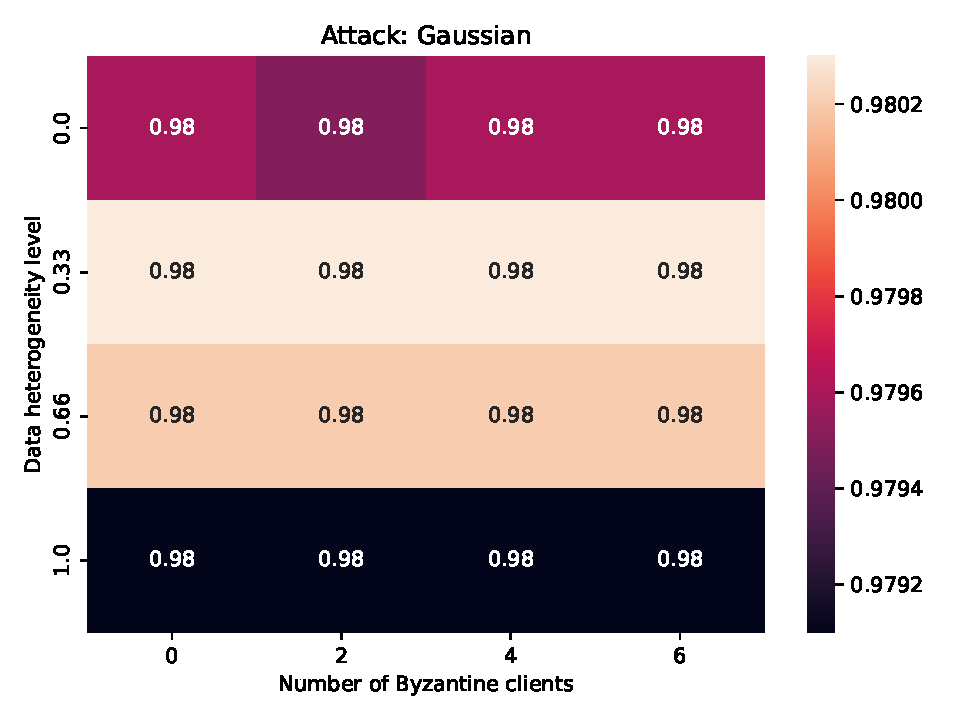
\includegraphics[width=\textwidth]{cnn_complete_plots/best_test_Gaussian_mnist_convnet_cnn_gamma_similarity_niid_NNM_ARC_nb_honest_clients_16_tolerated_f_equal_real.pdf}
        \caption{CNN (Gaussian Attack)}
        \label{fig:gaussian_cnn}
    \end{subfigure}
    \hfill
    \begin{subfigure}[b]{0.49\textwidth}
        \centering
        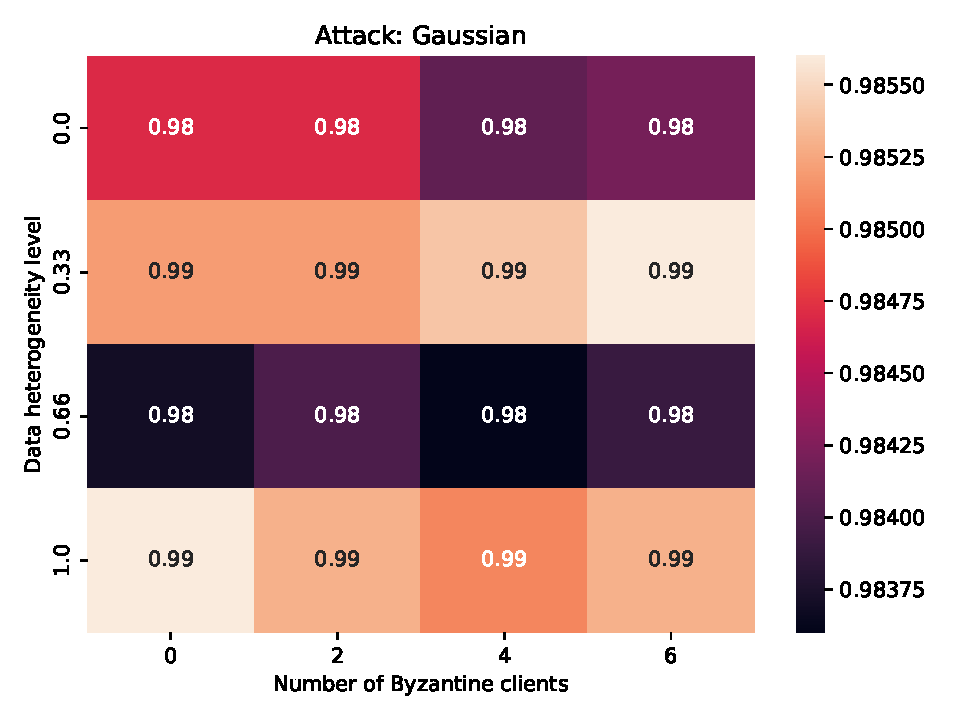
\includegraphics[width=\textwidth]{snn_complete_plots_rate/best_test_Gaussian_mnist_convnet_snn_gamma_similarity_niid_NNM_ARC_nb_honest_clients_16_tolerated_f_equal_real.pdf}
        \caption{SNN Rate (Gaussian Attack)}
        \label{fig:gaussian_snn_rate}
    \end{subfigure}
    
    \vspace{15pt}
    
    \begin{subfigure}[b]{0.49\textwidth}
        \centering
        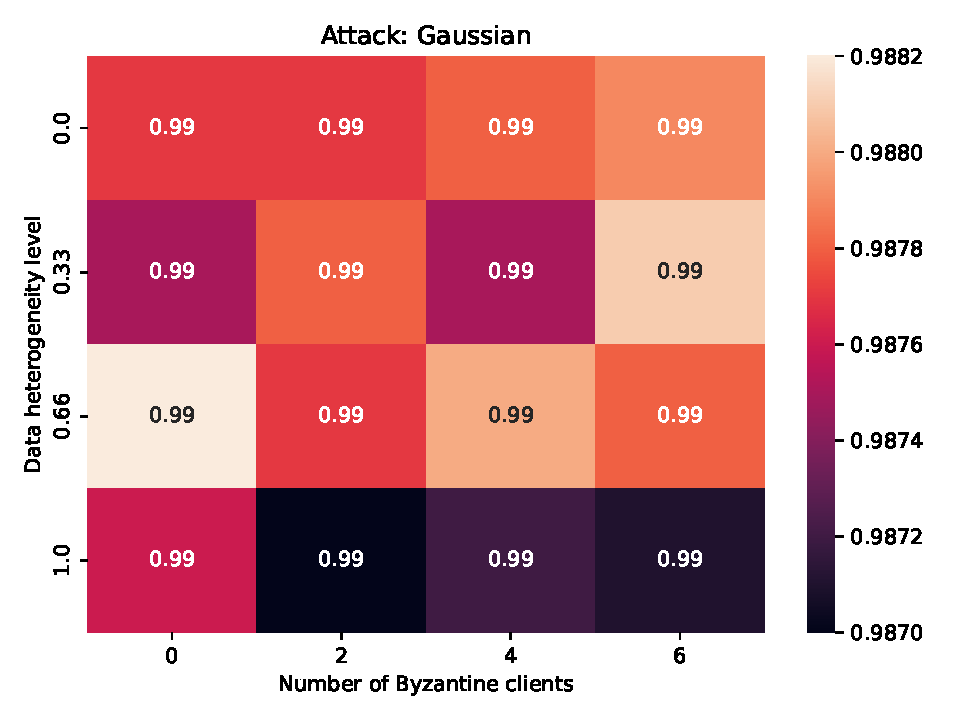
\includegraphics[width=\textwidth]{snn_complete_plots_direct/best_test_Gaussian_mnist_convnet_snn_gamma_similarity_niid_NNM_ARC_nb_honest_clients_16_tolerated_f_equal_real.pdf}
        \caption{SNN Direct (Gaussian Attack)}
        \label{fig:gaussian_snn_direct}
    \end{subfigure}
    \hfill
    \begin{subfigure}[b]{0.49\textwidth}
        \centering
        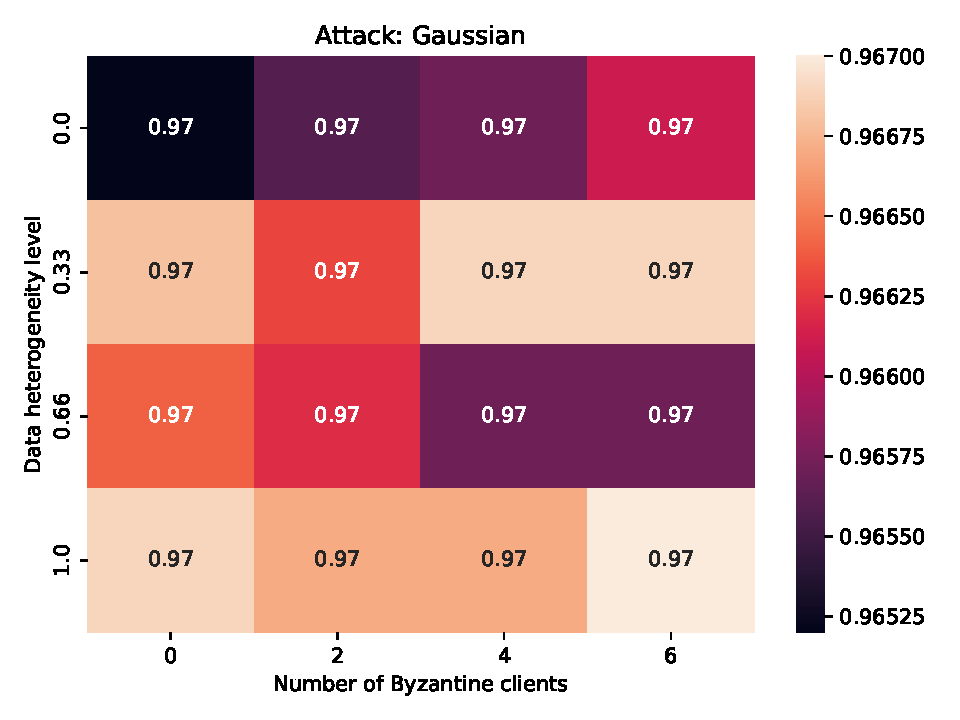
\includegraphics[width=\textwidth]{snn_complete_plots_nmnist/best_test_Gaussian_nmnist_nmnist_snn_gamma_similarity_niid_NNM_ARC_nb_honest_clients_16_tolerated_f_equal_real.pdf}
        \caption{SNN NMNIST (Gaussian Attack)}
        \label{fig:gaussian_snn_nmnist}
    \end{subfigure}
    \caption{Accuracy comparison under Gaussian attack across different data distribution parameters and number of Byzantine clients.}
    \label{fig:gaussian_attack}
\end{figure}

\newpage

\section{Fixed Attack: Optimal A Little Is Enough (ALIE)}
\label{sec:alie_attack}

Figure~\ref{fig:alie_attack} compares performance under the Optimal A Little Is Enough (ALIE) attack.

\begin{figure}[htbp]
    \centering
    \begin{subfigure}[b]{0.49\textwidth}
        \centering
        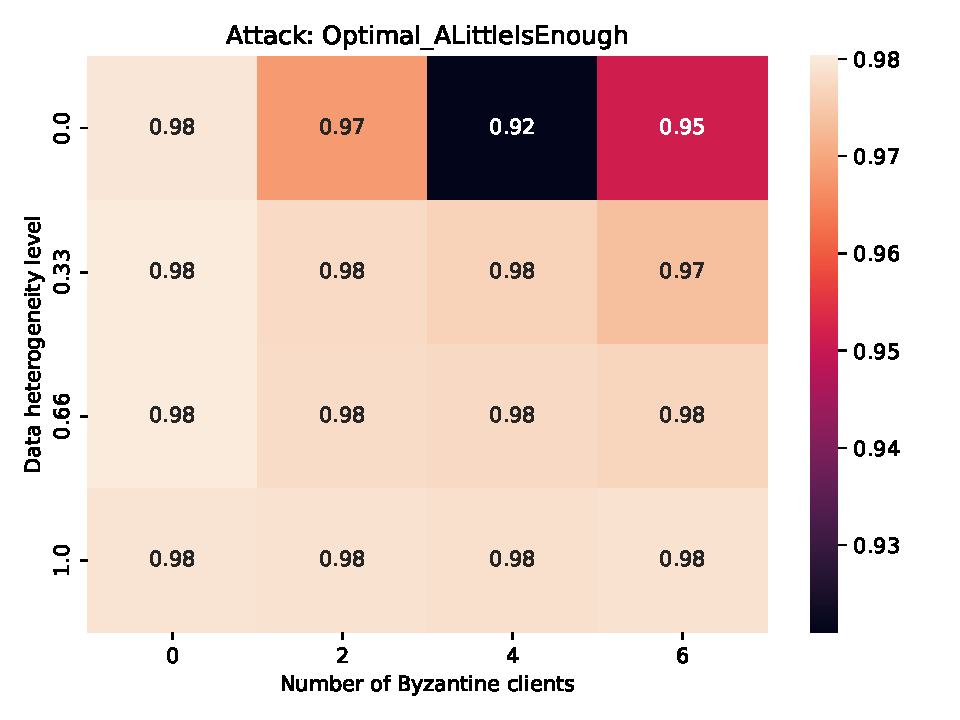
\includegraphics[width=\textwidth]{cnn_complete_plots/best_test_Optimal_ALittleIsEnough_mnist_convnet_cnn_gamma_similarity_niid_NNM_ARC_nb_honest_clients_16_tolerated_f_equal_real.pdf}
        \caption{CNN (ALIE Attack)}
        \label{fig:alie_cnn}
    \end{subfigure}
    \hfill
    \begin{subfigure}[b]{0.49\textwidth}
        \centering
        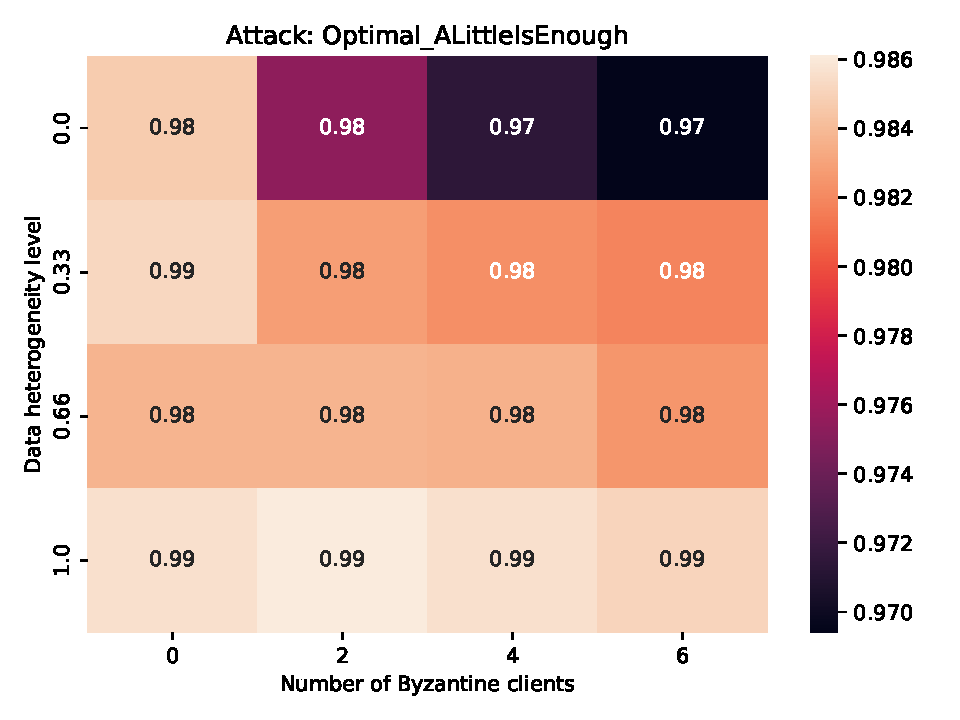
\includegraphics[width=\textwidth]{snn_complete_plots_rate/best_test_Optimal_ALittleIsEnough_mnist_convnet_snn_gamma_similarity_niid_NNM_ARC_nb_honest_clients_16_tolerated_f_equal_real.pdf}
        \caption{SNN Rate (ALIE Attack)}
        \label{fig:alie_snn_rate}
    \end{subfigure}
    
    \vspace{15pt}
    
    \begin{subfigure}[b]{0.49\textwidth}
        \centering
        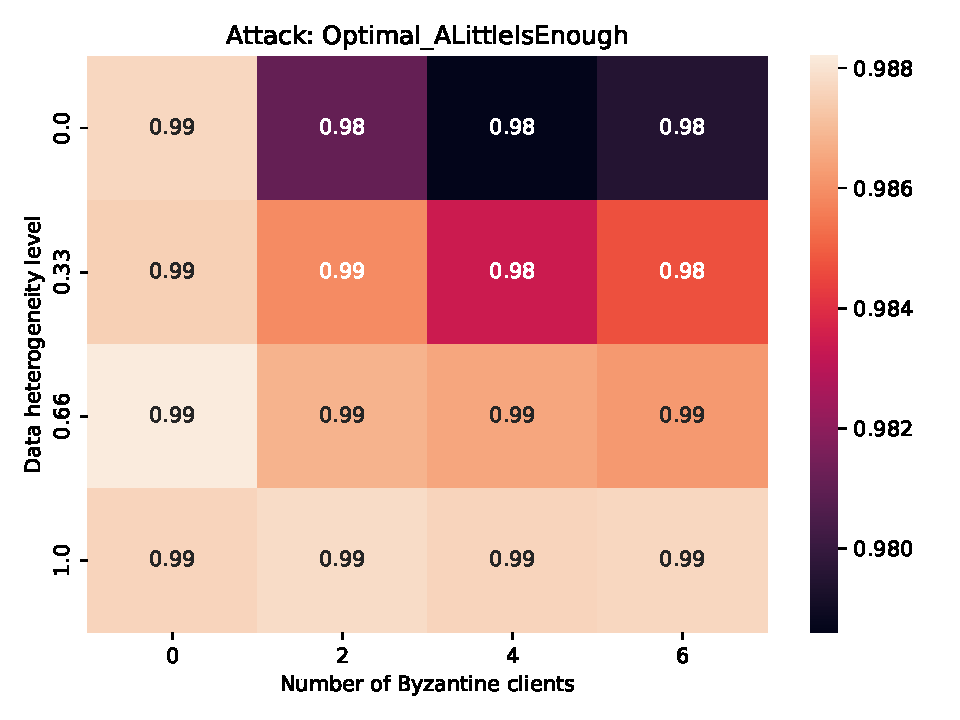
\includegraphics[width=\textwidth]{snn_complete_plots_direct/best_test_Optimal_ALittleIsEnough_mnist_convnet_snn_gamma_similarity_niid_NNM_ARC_nb_honest_clients_16_tolerated_f_equal_real.pdf}
        \caption{SNN Direct (ALIE Attack)}
        \label{fig:alie_snn_direct}
    \end{subfigure}
    \hfill
    \begin{subfigure}[b]{0.49\textwidth}
        \centering
        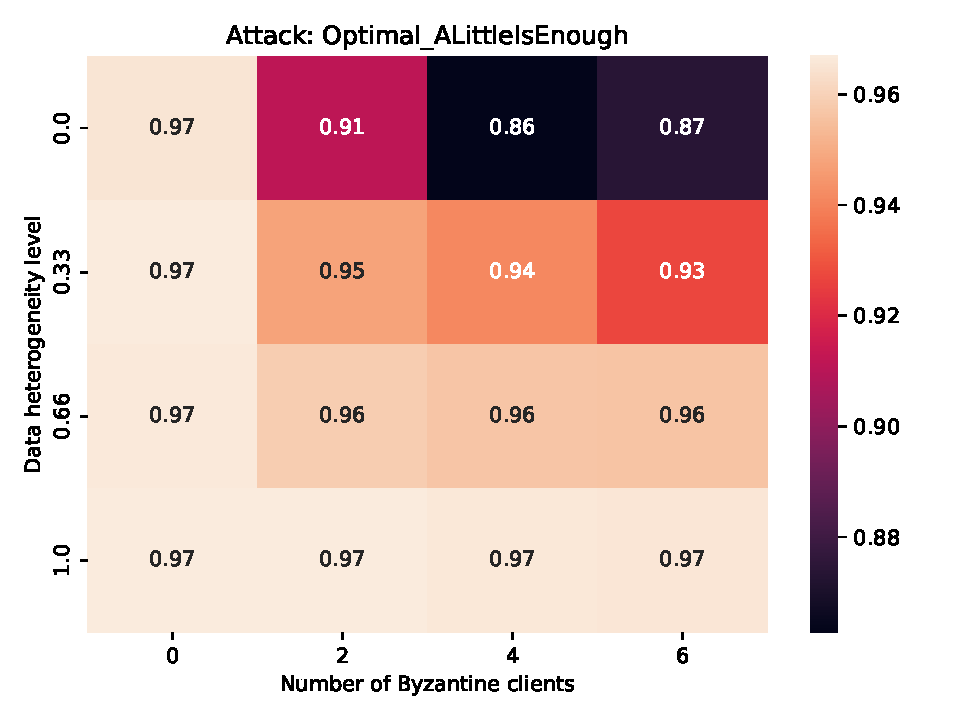
\includegraphics[width=\textwidth]{snn_complete_plots_nmnist/best_test_Optimal_ALittleIsEnough_nmnist_nmnist_snn_gamma_similarity_niid_NNM_ARC_nb_honest_clients_16_tolerated_f_equal_real.pdf}
        \caption{SNN NMNIST (ALIE Attack)}
        \label{fig:alie_snn_nmnist}
    \end{subfigure}
    \caption{Accuracy comparison under Optimal ALIE attack across different data distribution parameters and number of Byzantine clients.}
    \label{fig:alie_attack}
\end{figure}

\newpage

\section{Fixed Attack: Optimal Inner Product Manipulation (IPM)}
\label{sec:ipm_attack}

Figure~\ref{fig:ipm_attack} compares performance under the Optimal Inner Product Manipulation (IPM) attack.

\begin{figure}[htbp]
    \centering
    \begin{subfigure}[b]{0.49\textwidth}
        \centering
        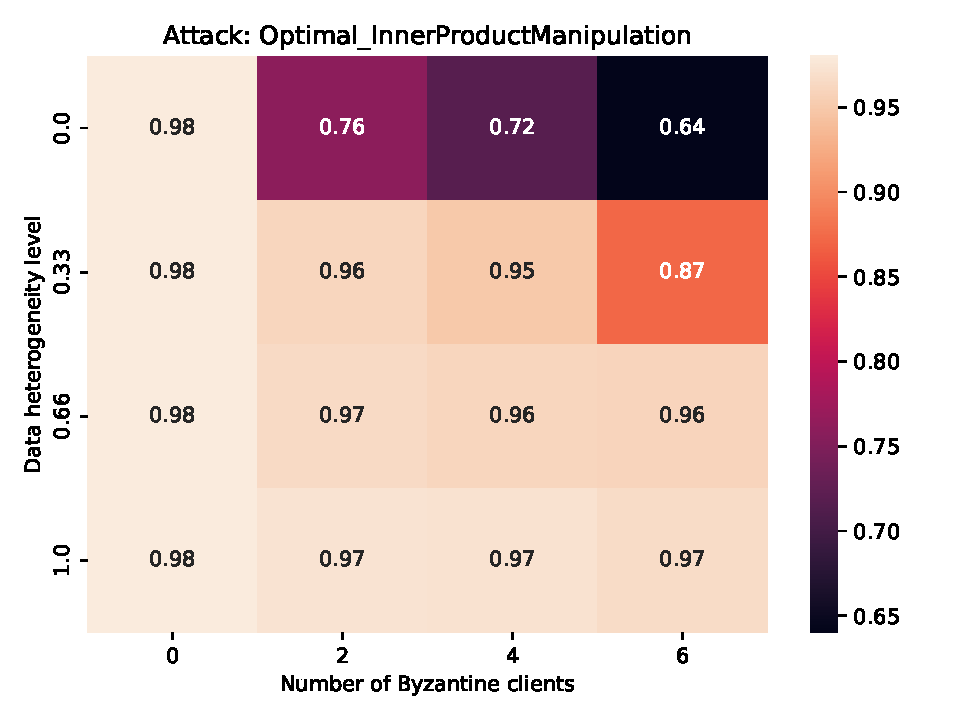
\includegraphics[width=\textwidth]{cnn_complete_plots/best_test_Optimal_InnerProductManipulation_mnist_convnet_cnn_gamma_similarity_niid_NNM_ARC_nb_honest_clients_16_tolerated_f_equal_real.pdf}
        \caption{CNN (IPM Attack)}
        \label{fig:ipm_cnn}
    \end{subfigure}
    \hfill
    \begin{subfigure}[b]{0.49\textwidth}
        \centering
        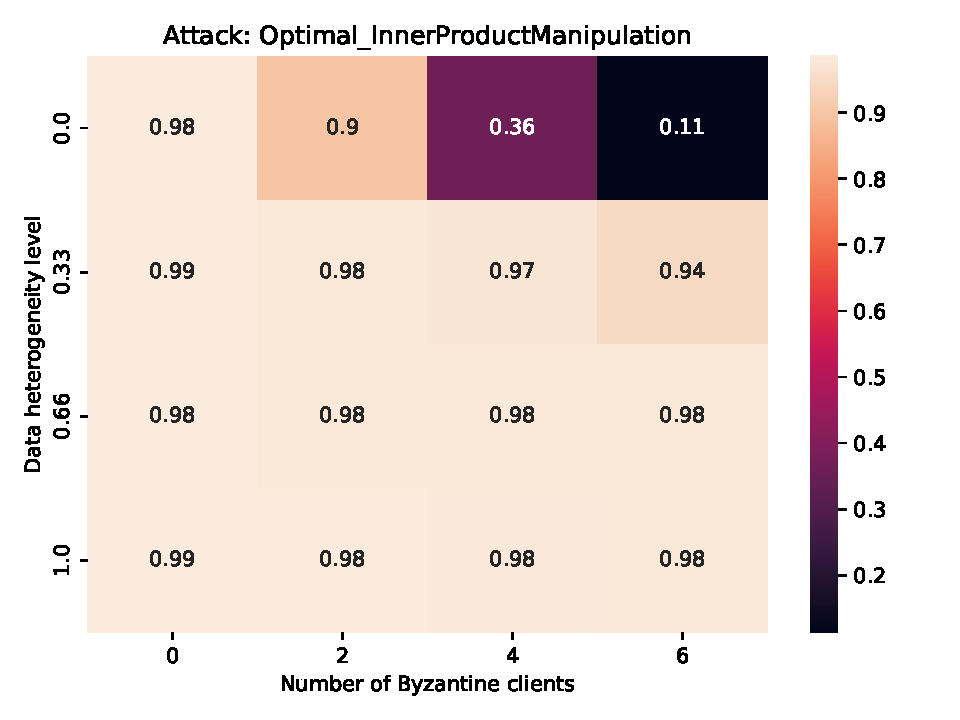
\includegraphics[width=\textwidth]{snn_complete_plots_rate/best_test_Optimal_InnerProductManipulation_mnist_convnet_snn_gamma_similarity_niid_NNM_ARC_nb_honest_clients_16_tolerated_f_equal_real.pdf}
        \caption{SNN Rate (IPM Attack)}
        \label{fig:ipm_snn_rate}
    \end{subfigure}
    
    \vspace{15pt}
    
    \begin{subfigure}[b]{0.49\textwidth}
        \centering
        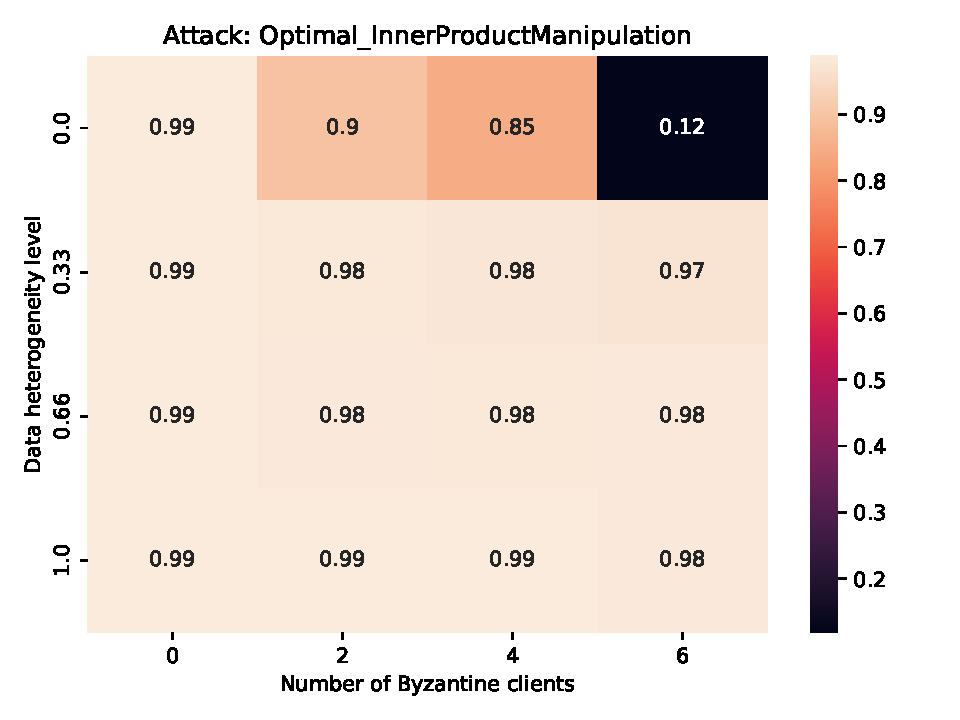
\includegraphics[width=\textwidth]{snn_complete_plots_direct/best_test_Optimal_InnerProductManipulation_mnist_convnet_snn_gamma_similarity_niid_NNM_ARC_nb_honest_clients_16_tolerated_f_equal_real.pdf}
        \caption{SNN Direct (IPM Attack)}
        \label{fig:ipm_snn_direct}
    \end{subfigure}
    \hfill
    \begin{subfigure}[b]{0.49\textwidth}
        \centering
        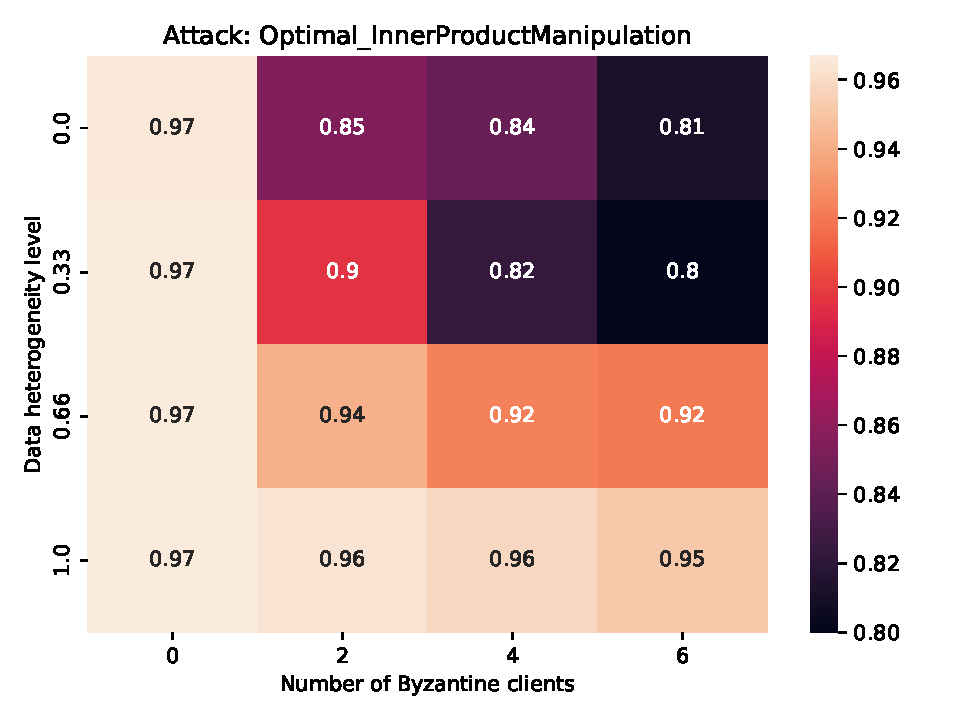
\includegraphics[width=\textwidth]{snn_complete_plots_nmnist/best_test_Optimal_InnerProductManipulation_nmnist_nmnist_snn_gamma_similarity_niid_NNM_ARC_nb_honest_clients_16_tolerated_f_equal_real.pdf}
        \caption{SNN NMNIST (IPM Attack)}
        \label{fig:ipm_snn_nmnist}
    \end{subfigure}
    \caption{Accuracy comparison under Optimal IPM attack across different data distribution parameters and number of Byzantine clients.}
    \label{fig:ipm_attack}
\end{figure}

\newpage

\section{Fixed Attack: Sign Flipping}
\label{sec:sign_flipping_attack}

Figure~\ref{fig:sign_flipping_attack} compares performance under the Sign Flipping attack.

\begin{figure}[htbp]
    \centering
    \begin{subfigure}[b]{0.49\textwidth}
        \centering
        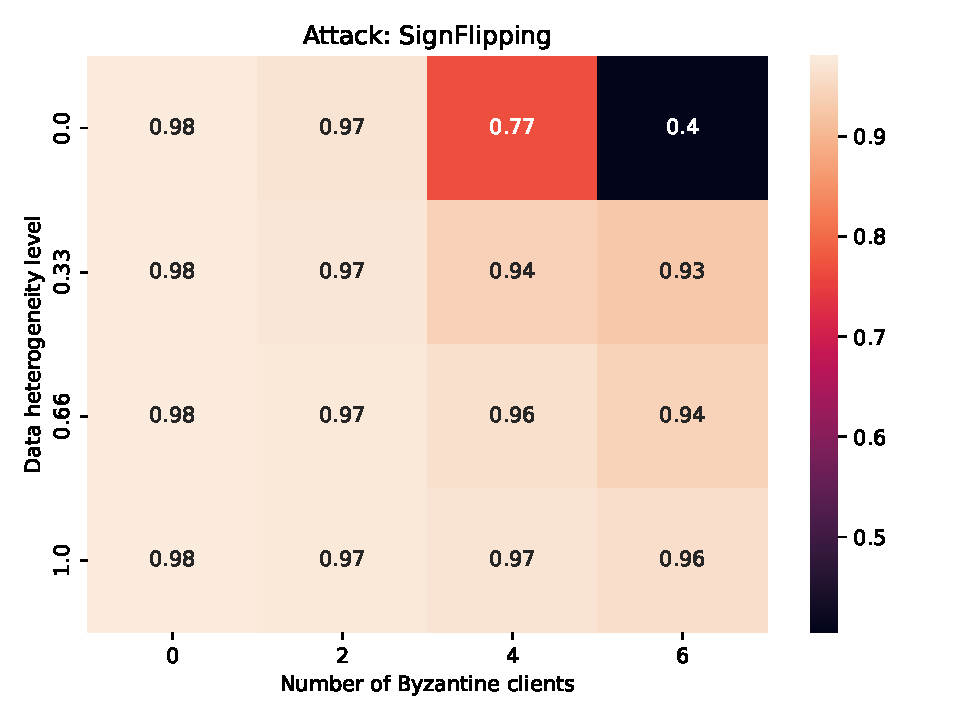
\includegraphics[width=\textwidth]{cnn_complete_plots/best_test_SignFlipping_mnist_convnet_cnn_gamma_similarity_niid_NNM_ARC_nb_honest_clients_16_tolerated_f_equal_real.pdf}
        \caption{CNN (Sign Flipping)}
        \label{fig:sf_cnn}
    \end{subfigure}
    \hfill
    \begin{subfigure}[b]{0.49\textwidth}
        \centering
        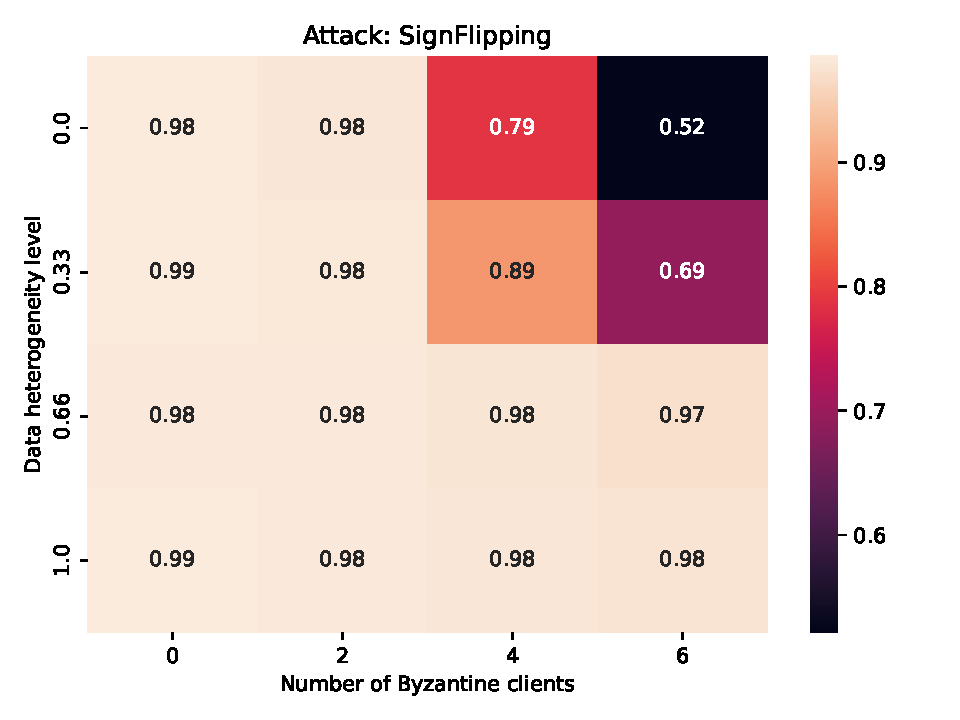
\includegraphics[width=\textwidth]{snn_complete_plots_rate/best_test_SignFlipping_mnist_convnet_snn_gamma_similarity_niid_NNM_ARC_nb_honest_clients_16_tolerated_f_equal_real.pdf}
        \caption{SNN Rate (Sign Flipping)}
        \label{fig:sf_snn_rate}
    \end{subfigure}
    
    \vspace{15pt}
    
    \begin{subfigure}[b]{0.49\textwidth}
        \centering
        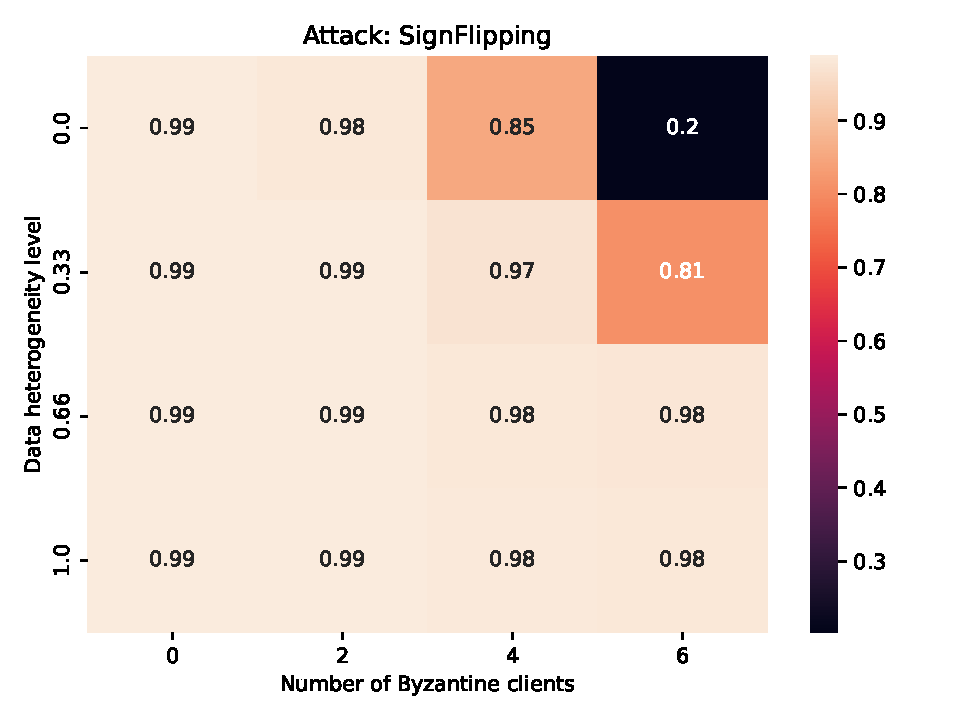
\includegraphics[width=\textwidth]{snn_complete_plots_direct/best_test_SignFlipping_mnist_convnet_snn_gamma_similarity_niid_NNM_ARC_nb_honest_clients_16_tolerated_f_equal_real.pdf}
        \caption{SNN Direct (Sign Flipping)}
        \label{fig:sf_snn_direct}
    \end{subfigure}
    \hfill
    \begin{subfigure}[b]{0.49\textwidth}
        \centering
        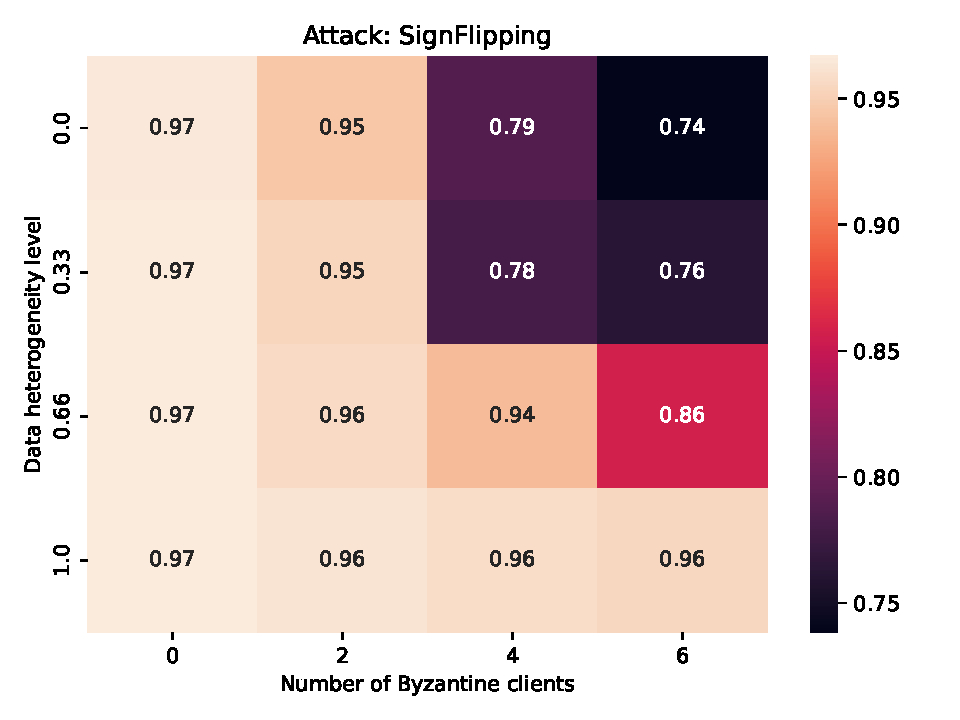
\includegraphics[width=\textwidth]{snn_complete_plots_nmnist/best_test_SignFlipping_nmnist_nmnist_snn_gamma_similarity_niid_NNM_ARC_nb_honest_clients_16_tolerated_f_equal_real.pdf}
        \caption{SNN NMNIST (Sign Flipping)}
        \label{fig:sf_snn_nmnist}
    \end{subfigure}
    \caption{Accuracy comparison under Sign Flipping attack across different data distribution parameters and number of Byzantine clients.}
    \label{fig:sign_flipping_attack}
\end{figure}

\end{document}
